\chapter{Index Analysis of the MNA}

%seite 22 kap 7 netw top and dae ind for rlc - modelling and discretization circ prob
\cite{ModellingAndDiscretizationOfCircuitProblems}

In the previous chapter we have seen two different kinds of Index concepts for differential algebraic equations. We have also seen that these two, even though they describe rather different structural aspects of the equation, are identical for our use-cases. This leads to the question, what indices we expect obtain for our MNA system.

This chapter aims to answer that question for the linear case of circuits only containing resistors, inductors and capacities (RLC). Linear means that the RLC components are described by linear functions with positive capacitances, inductances and resistances. Thus the matrices
\begin{displaymath}
	C:=\frac{\partial q_C(w)}{\partial w}, \quad L:=\frac{\partial \phi_L(w)}{\partial w}, \quad G:=\frac{\partial r(w)}{\partial w}
\end{displaymath}
are positive definite and symmetric. The generalization of these results to the nonlinear case still relies on positive definiteness.

Recall that we consider the equations resulting from the analysis above. These equations are of the form \eqref{DAE-const-coeff}:
\begin{displaymath}
	A y'(t) + B y(t) = f(t).
\end{displaymath}
Specifically the obtained equations from section \ref{MNA_Matrixform} are
\begin{displaymath}
	\begin{pmatrix}
		A_C C A_C^\top & 0 & 0 \\
		0 & L & 0 \\
		0 & 0 & 0
	\end{pmatrix}
	*
	\begin{pmatrix}
		\dot{u} \\
		\dot{i_L} \\
		\dot{i_V}
	\end{pmatrix}
	+
	\begin{pmatrix}
		A_R G A_R^\top & A_L & A_V \\
		-A_L^\top & 0 & 0 \\
		-A_V^\top & 0 & 0 ä
	\end{pmatrix}
	*
	\begin{pmatrix}
		u \\
		i_L \\
		i_V
	\end{pmatrix}
	=
	\begin{pmatrix}
		-A_I i_{src} \\
		0 \\
		-v_{src}
	\end{pmatrix}.
\end{displaymath}

\section{General Index analysis}

Assuming the system only contains linear elements, or is linearized at an operating point in order to investigate the system behaviour, then the corresponding network equation represents a DAE with constant coefficients \eqref{DAE-const-coeff}. We denote $x(t)=(u(t), i_L(t), i_V(t))^\top$. The structure of the system is reliant on the matrix $B$, thus we consider two cases

\paragraph{ODE-case:}
	The matrix $B$ in \eqref{DAE-const-coeff} is regular. This is the case iff the circuit contains no voltage sources and there are no nodes which have no path to ground via capacitors. Then the system represents a linear-implicit system of ODEs and can be transformed into the explicit ODE sytstem
	\begin{displaymath}
		\dot{x}=B^{-1}(-Ax+f(t)).
	\end{displaymath}
	Thus we obtain an index of $0$.
		
\paragraph{DAE-case:}
	The matrix $B$  in \eqref{DAE-const-coeff} is singular. This is the interesting case which we will analyse in the following.


For the singular matrix $B$ we have already obtained a representation of the form
\begin{align*}
	u'(t) + Ru(t) &= s(t), \\
	Nv'(t) + v(t) &= q(t)
\end{align*}
in the previous section, see \eqref{transformed-DAE-const-coeff}. We now consider the nilpotency index $\nu$ of the matrix $N$, since we already know that this index correlates with the differentiation as well as the perturbation index. We consider two cases:

\begin{enumerate}
	\item \textbf{The nilpotency index is 1} \newline
		Because $N$ is nilpotent with nipotency index $\nu = 1$ it holds that $N^1 = 0$, thus the system transforms to
		\begin{align*}
			u'(t) + Ru(t) &= s(t), \\
			v(t) &= q(t).
		\end{align*}
		This means that the algebraic variables are given explicitly. Thus the system is in ODE form.

	\item \textbf{The nilpotency index is $\geq$ 2} \newline
		This case is the situation we have seen in section \ref{chap:Weierstraß-Kronecker Normalform}, it led to \eqref{solution-to-transformed-DAE-const-coeff-part2}
		\begin{displaymath}
			v(t) = \sum_{i=0}^{\nu-1} (-1)^iN^iq^{(i)}(t).
		\end{displaymath}
		By differentiating the above equation one more time, we obtain
		\begin{equation}
			v'(t) = \sum_{i=0}^{\nu-1} (-1)^iN^iq^{(i+1)}(t)
		\end{equation}
		with the assumption that $q$ is $\nu$ times differentiable.
\end{enumerate}

We can see that the solution has to fulfill an algebraic constraint. In the case of index $\nu = 1$ this equation is given explicitly, while for index $\nu \geq 2$ it is given implicitly.

The system is also sensitive to perturbations. Small noise in the input can have arbitrarily large derivatives which can influence $v$ as we it depends on them.

This means no severe numerical problems arise from index-1 systems. Implicit numerical integration schemes for stiff systems are feasable. On the other hand severe nunmerical problems may occur in the case that the system has index greater or equal to $2$. The hidden constraints can only be resolved by an unstable differentiation process.

As the Kronecker index $k=ind\{A,B\}$ defines the behaviour of the system theoretically as well as numerically it is called the \emph{algebraic index} of the linear implicit system.

\section{Topological Conditions} 
\cite{Tischendorf2005Topological}, %chapter 7 of
\cite{ModellingAndDiscretizationOfCircuitProblems}
\cite{DesoerCharlesA1969Bct}

From analyzing the MNA some conditions to the circuit topology can be obtained. We will be considering the impact of special arrangements of components on the index of the system. In \cite{Tischendorf2005Topological} they present very interesting results about the index of MNA equations.


\begin{theorem}[Index-1 condition \cite{Tischendorf2005Topological}] \label{Index-1 condition}
	Let the matrices of the capacitances, inductances and resistances be positive definite. If the network neither cointains \emph{inductance-current-source cutsets} nor (controlled?) \emph{capacitance-voltage-source loops}, then the MNA leads to an index-1 DAE.
\end{theorem}

Where inductance-current-source cutsets and capacitance-voltage-source loops are subcircuits of the form (Seite 481 (searchbar) in basic circuit theory)

\begin{figure}[H]
	\begin{subfigure}{0.5\textwidth}
		\centering
		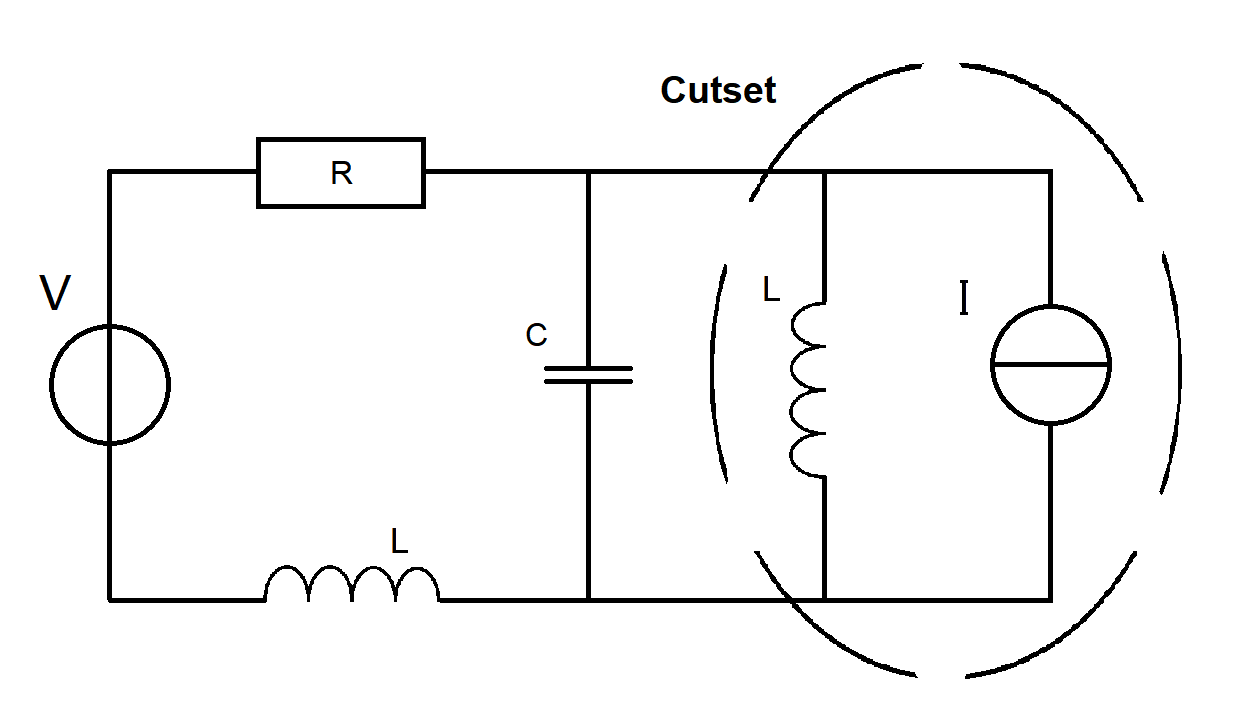
\includegraphics[width=0.9\linewidth]{pictures/inductance-current-source_cutset.png}
		\caption{inductance-current-source cutset}
	\end{subfigure}
	\begin{subfigure}{0.5\textwidth}
		\centering
		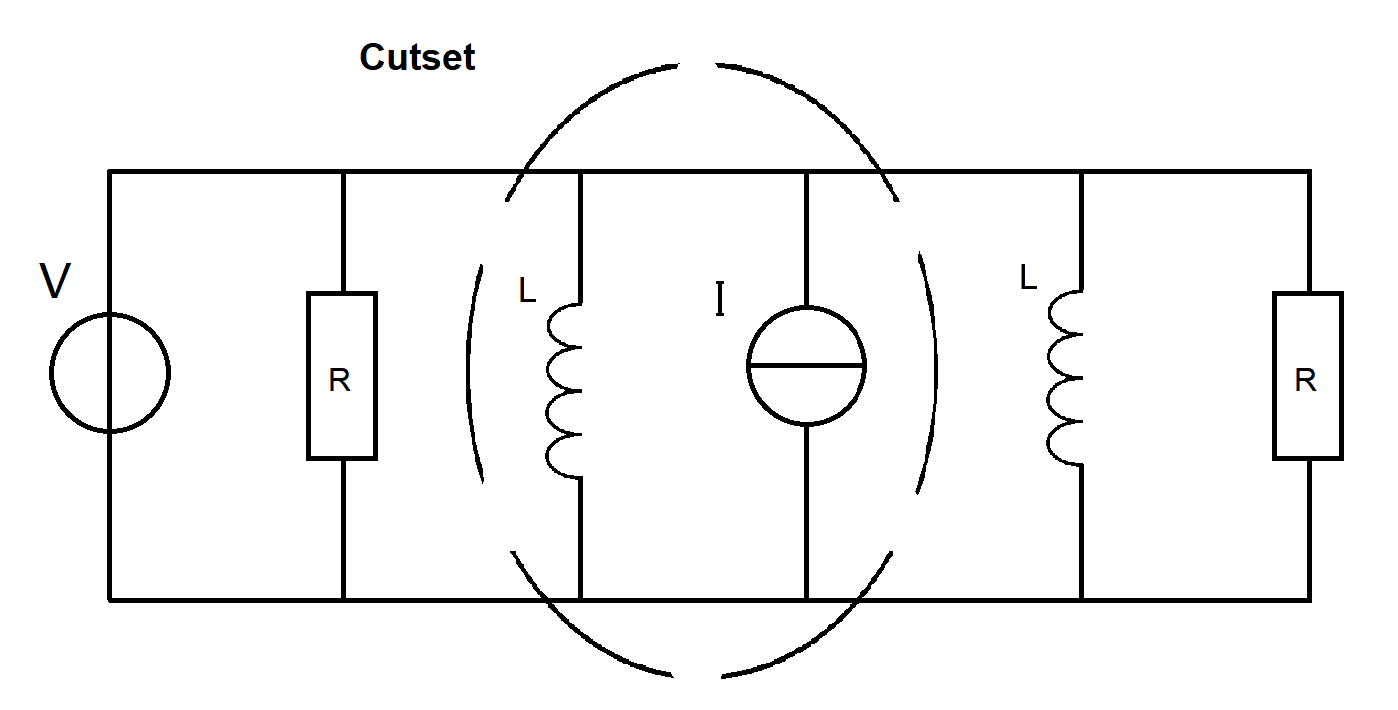
\includegraphics[width=0.9\linewidth]{pictures/capacitance-voltage-source_loop.png}
		\caption{capacitance-voltage-source loop}
	\end{subfigure}
	\label{cutset and loop}
	\caption{cutset and loop}
\end{figure}

This means that if our circuit does not contain any loops or cutsets of the above form the resulting MNA system has index 1.

\begin{theorem}[Index-2 condition \cite{Tischendorf2005Topological}] \label{Index-2 condition}
	If the Network contains \emph{inductance-current-source cutsets} or \emph{capacitance-voltage-source loops} except for capacitance-only loops, then the MNA leads to an index-2 DAE.
\end{theorem}

These results can also be interpreted in a more formal way. As they are just descriptions of the topology of the circuit we can reformulate the theorems in terms of the incidence matrix $A$.

By perturbing the right hand side of of \eqref{MNA_Matrixform} with a slight perturbation $\delta = (\delta_C, \delta_L, \delta_V)^\top$ we get a corresponding solution $x^\delta = (u^\delta, i_l^\delta, i_V^\delta)^\top$. One can show that the difference of this perturbed solution to the solution $x$ of the unperturbed system is bounded by
\begin{displaymath}
	|| x^\delta - x(t) || \leq C * \left( ||x^\delta (0) - x(0)|| + \max_{0 \leq \tau \leq t} ||\delta(\tau)|| + \max_{0 \leq \tau \leq t} ||Q_{CRV}^\top \dot{\delta_C}|| + \max_{0 \leq \tau \leq t} ||\tilde{Q}_{V-C}^\top \dot{\delta_V}|| \right)
\end{displaymath}

using orthogonal projectors$Q_C$, $Q_{CRV}$ and $\tilde{Q}_{V-C}$  onto $ker(A_C^\top)$, $ker(A_CA_RA_V)^\top$ and $ker(Q_C^\top A_V)$ respectively. We denot $ker(A) = \{x: Ax = 0\}$.

Hence, Theorem \ref{Index-1 condition} can be interpreted as the two conditions

\begin{equation}
	\label{eq:alt-condditions}
	\begin{aligned}
		kerQ_C^\top A_v &= {0}, \\
		ker(A_C A_R A_V)^\top &= {0}.
	\end{aligned}
\end{equation}
	

This means that for ``reasonable'' RLC circuits, i.e. circuits satisfying the prerequisites of the above Theorem \ref{Index-1 condition}, the index will not exceed 2. We will only consider such circuits in this thesis.

If one of the conditions \eqref{eq:alt-condditions} is violated, we are in the case of Theorem \ref{Index-2 condition} and thus have index 2.

We will apply those results to some examples: %(there are examples on page 23)

\textbf{examples}